\documentclass[a4paper]{article}

\usepackage{polski}
\usepackage[utf8]{inputenc}
\usepackage{graphicx}
\usepackage[hidelinks]{hyperref}
\usepackage{listings}
\usepackage{multirow}
\usepackage{color}
\usepackage[labelformat=empty]{caption}

\definecolor{lbcolor}{rgb}{0.9,0.9,0.9}
\lstset{
    inputencoding=utf8, 
    extendedchars=true,
   	language=Perl,
    backgroundcolor=\color{lbcolor},
	basicstyle=\small\scriptsize,
	frame=tb,
	showstringspaces=false,
	commentstyle=\color{red},
	keywordstyle=\color{blue},
    literate={ą}{{\k{a}}}1
             {Ą}{{\k{A}}}1
             {ę}{{\k{e}}}1
             {Ę}{{\k{E}}}1
             {ó}{{\'o}}1
             {Ó}{{\'O}}1
             {ś}{{\'s}}1
             {Ś}{{\'S}}1
             {ł}{{\l{}}}1
             {Ł}{{\L{}}}1
             {ż}{{\.z}}1
             {Ż}{{\.Z}}1
             {ź}{{\'z}}1
             {Ź}{{\'Z}}1
             {ć}{{\'c}}1
             {Ć}{{\'C}}1
             {ń}{{\'n}}1
             {Ń}{{\'N}}1
}


\title{Zgłębianie danych - raport}
\author{Kacper Siora}
\date{\today}

\begin{document}
\maketitle

\section{Treść zadania}

\hspace{1cm}\textit{"Sprawdzić prawo Zipf’a w języku polskim: dla różnych grup dokumentów sporządzić listę występujących słów, uporządkować je wg częstości wystąpień (od najczęstszego) i sprawdzić wartości iloczynów r*f gdzie r jest rangą słowa (numerem na liście), f częstością wystąpień tego słowa. Dla języka angielskiego iloczyn ten wynosi ok. 0.1."}


\hspace{1cm} Prawo Zipf'a mówi, że w korpusie języka naturalnego, częstotliwość występowania słów jest odwrotnie proporcjonalna do pozycji w rankingu. Ranking powstaje w wyniku zliczenia częstotliwości występowania słów oraz posortowania malejąco powstałej listy. Prawo było

\hspace{1cm}Prawo to jest wszechoobecne w świecie i odeszło od sensu stricte lingwistycznego. Prawo Zipf'a może być pomocne przy ustalaniu \textit{tzw. stoplist (ang. stopwords list)}. Ponadto przydatne jest w takich sytuacjach jak: liczba ludności w miastach, częstość nazwisk w książce telefonicznej, rozkład trzęsień Ziemi.


\section{Narzędzia}
\hspace{1cm}Aby zliczyć ilość słów oraz częstość ich występowania postanowiłem skorzystać z systemu zarządzania bazą danych MongoDB. Korzystałem również ze skryptu perl, oraz programu tr w systemie Linux. 
\section{Dane}
\hspace{1cm}Dokumenty, których używałem w projekcie to:
\begin{itemize}
\item \textit{Alicja w Krainie Czarów}
\item \textit{Nad Niemnem}
\item \textit{W pustyni i w puszczy}
\item \textit{Pianista}
\item \textit{Ewangelia wg św. Mateusza}
\item \textit{Regulamin studiów Uniwersytetu Gdańskiego}
\item \textit{Zbiór tekstów z płyty  „Marek Grechuta \& Anawa”}
\item \textit{Treny J. Kochanowskiego}
\end{itemize}


\subsection{Przygotowanie danych}
\hspace{1cm}Po ściągnięciu wszystkich ww. dokumentów, musiałem odpowiednio je odpowiednio przerobić.

\begin{figure}[h!]
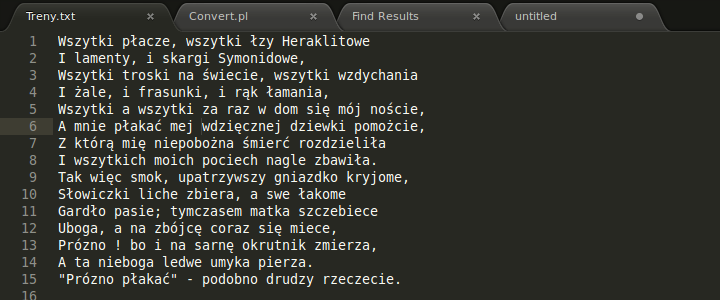
\includegraphics[width=1\textwidth]{treny.png}
\caption{\textit{Przykładowy dokument przed użyciem skryptu}}
\end{figure}

\hspace{1cm}Przy pomocy poniższego skryptu usunąłem wszelkie niepotrzebne znaki oraz pozbyłem się cyfr i polskich liter.  
\begin{lstlisting}
#!/usr/bin/perl

while (<>) {
    s/<.*>//;               # usuwanie < >
    s/\[//g;                # usuwanie [ ]
    s/\]//g;
    $_=" $_ ";              
    tr/A-Z/a-z/;            # zamiana na małe litery
    s/([0-9]*)//g;          # usuwanie liczb
    s/ą/a/g;                # zamiana polskich znaków
    s/Ą/a/g;
    s/ć/c/g;
    s/Ć/c/g;
    s/ę/e/g;
    s/Ę/e/g;
    s/ł/l/g;
    s/Ł/l/g;
    s/ń/n/g;
    s/Ń/n/g;
    s/ó/o/g;
    s/Ó/o/g;
    s/ś/s/g;
    s/Ś/s/g;
    s/ż/z/g;
    s/Ż/z/g;
    s/ź/z/g;
    s/Ź/z/g;
    tr/a-z/ /cs;
    chop;
    print $_;
}
\end{lstlisting}

\newpage
 
\begin{figure}[h!]
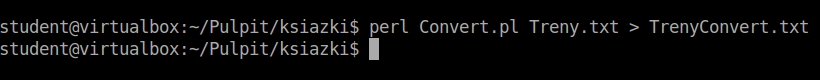
\includegraphics[width=1\textwidth]{convert_perl.png}
\caption{\textit{Komenda wykonująca skrypt}}
\end{figure}

\hspace{1cm}Po wykonaniu skryptu, z dokumentu usunięte zostały wszystkie znaki specjalne, cyfry oraz znaki interpunkcyjne. Dokument został zapisany słowo po słowie oddzielone spacjami w jednej linijce.

\begin{figure}[h!]
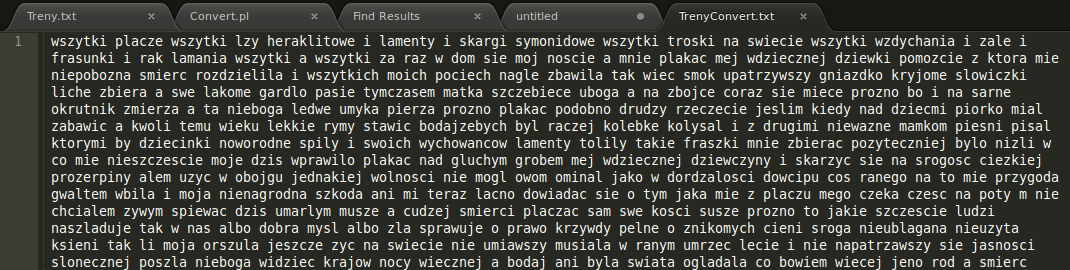
\includegraphics[width=1\textwidth]{treny_convert.png}
\caption{\textit{Przykładowy dokument po przerobieniu skryptem}}
\end{figure}

\hspace{1cm}Przed importem do bazy Mongo należy wykonać jeszcze jedną komendę. Dzięki programowi \textit{tr} każde słowo w naszym dokumencie zostanie zapisane w oddzielnej linijce.

\begin{figure}[h!]
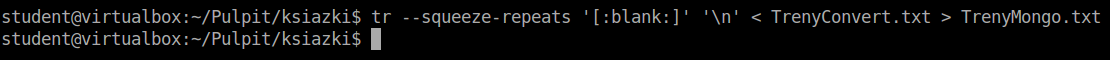
\includegraphics[width=1\textwidth]{treny_mongo.png}
\caption{\textit{Użycie programu tr do kolejnej konwersji dokumentu}}
\end{figure}



\begin{figure}[h!]
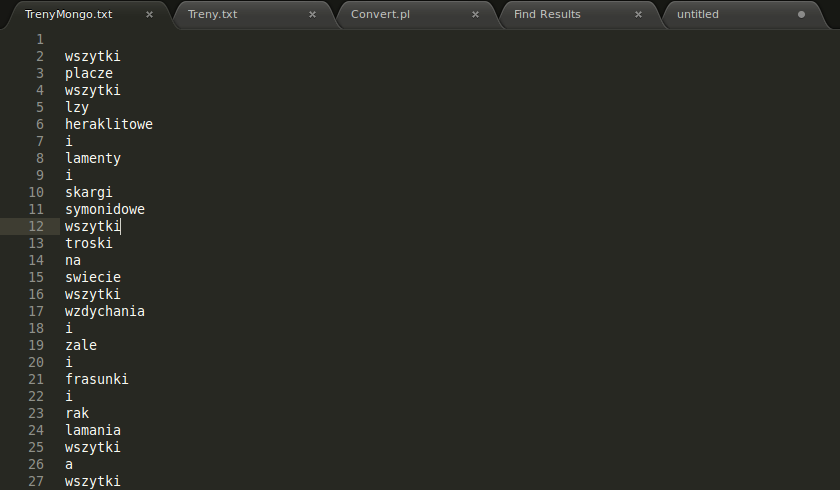
\includegraphics[width=1\textwidth]{treny_mongo2.png}
\caption{\textit{Przykładowy dokument po konwersji programem tr}}
\end{figure}




\subsection {Import danych}
\hspace{1cm}Tak przygotowane dane, możemy już importować do bazy danych Mongo. Aby zacząć pracę na systemie Windows wystarczy po prostu ściągnąć i rozpakować program ze strony producenta. Na sam początek musimy uruchomić program \textit{mongod.exe}

\begin{figure}[h!]
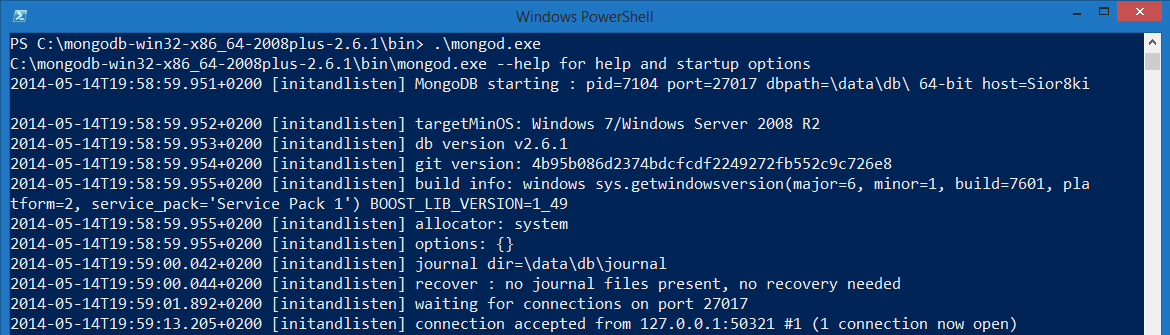
\includegraphics[width=1\textwidth]{mongod.png}
\caption{\textit{Uruchamianie usługi MongoDB daemon}}
\end{figure}

Teraz dopiero możemy zacząć import danych do bazy


\begin{figure}[h!]
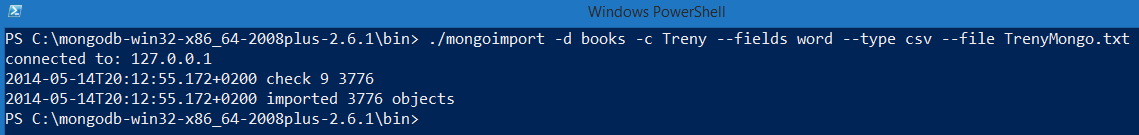
\includegraphics[width=1\textwidth]{treny_import.png}
\caption{\textit{Import danych do bazy}}
\end{figure}


Po zaimportowaniu wszystkich dokumentów możemy sprawdzić ile słów jest w danym tekście

\begin{figure}[h!]
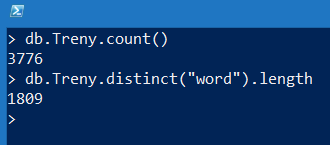
\includegraphics[width=1\textwidth]{treny_count.png}
\caption{\textit{Komenda MongoDB zwracająca ilość słów}}
\end{figure}


\section{Wyniki}


\hspace{1cm}Aby obliczyć \textit{f (częstość wystąpienia)} danego słowa, należy podzielić liczbę jego wystąpień przez ilość wszystkich słów w dokumencie.

\begin{figure}[h!]
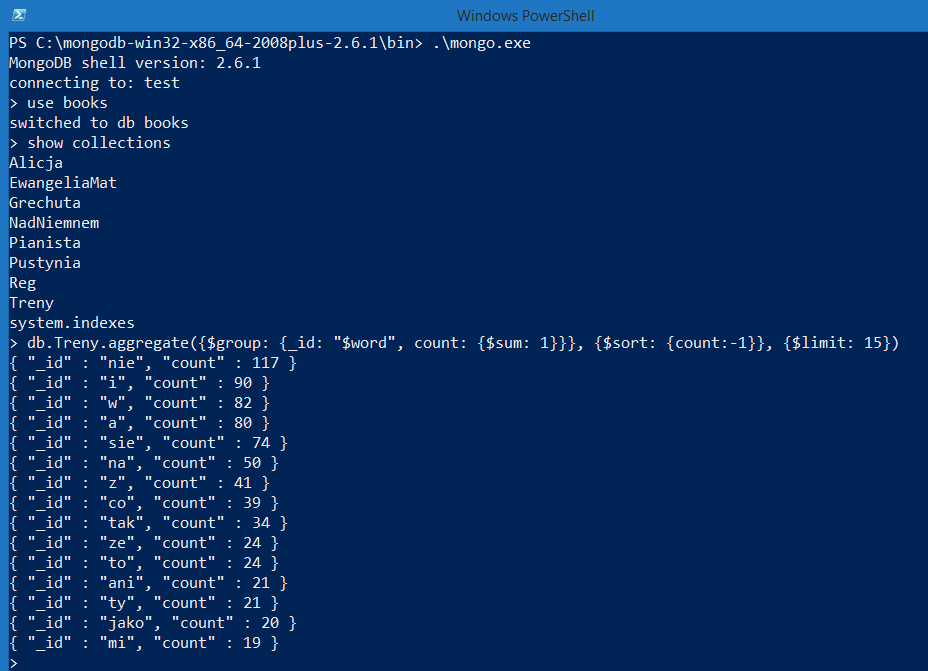
\includegraphics[width=1\textwidth]{treny_aggreate.png}
\caption{\textit{Wyszukiwanie najczęściej występujących słów}}
\end{figure}

\begin{table}
\begin{tabular}{|l|c|c|}
\hline
\textbf{Dokument}         & \textbf{Ilość wszystkich słów} & \textbf{Ilość słów różnych} \\ \hline
Alicja w Krainie Czarów   & 20018                          & 5495                        \\ \hline
Nad Niemnem               & 164352                         & 29677                       \\ \hline
W pustyni i w puszczy     & 100485                         & 17837                       \\ \hline
Pianista                  & 49201                          & 13590                       \\ \hline
Ewangelia wg św. Mateusza & 17455                          & 4287                        \\ \hline
Regulamin studiów         & 4798                           & 1267                        \\ \hline
Marek Grechuta \& Anawa   & 1718                           & 768                         \\ \hline
Treny J. Kochanowskiego   & 3776                           & 1809                        \\ \hline
\end{tabular}
\end{table}




\begin{table}
\begin{tabular}{ccc|c|l|}
\hline
\multicolumn{5}{|c|}{\textbf{Alicja w krainie czarów}}                                                                                                                            \\ \hline
\multicolumn{1}{|c|}{\textit{\textbf{r (rank)}}} & \multicolumn{1}{c|}{\textbf{słowo}}  & \textit{\textbf{ilość wystąpień}} & \textit{\textbf{f (częstość wystąpienia)}} & r * f  \\ \hline
\multicolumn{1}{|c|}{\textit{1}}                 & \multicolumn{1}{c|}{\textit{sie}}    & 655                               & 0,0327                                     & 0,0327 \\ \hline
\multicolumn{1}{|c|}{\textit{2}}                 & \multicolumn{1}{c|}{\textit{nie}}    & 494                               & 0,0247                                     & 0,0494 \\ \hline
\multicolumn{1}{|c|}{\textit{3}}                 & \multicolumn{1}{c|}{\textit{i}}      & 454                               & 0,0227                                     & 0,0680 \\ \hline
\multicolumn{1}{|c|}{\textit{4}}                 & \multicolumn{1}{c|}{\textit{w}}      & 409                               & 0,0204                                     & 0,0817 \\ \hline
\multicolumn{1}{|c|}{\textit{5}}                 & \multicolumn{1}{c|}{\textit{na}}     & 388                               & 0,0194                                     & 0,0969 \\ \hline
\multicolumn{1}{|c|}{\textit{6}}                 & \multicolumn{1}{c|}{\textit{alicja}} & 339                               & 0,0169                                     & 0,1016 \\ \hline
\multicolumn{1}{|c|}{\textit{7}}                 & \multicolumn{1}{c|}{\textit{ze}}     & 322                               & 0,0161                                     & 0,1126 \\ \hline
\multicolumn{1}{|c|}{\textit{8}}                 & \multicolumn{1}{c|}{\textit{z}}      & 319                               & 0,0159                                     & 0,1275 \\ \hline
\multicolumn{1}{|c|}{\textit{9}}                 & \multicolumn{1}{c|}{\textit{to}}     & 317                               & 0,0158                                     & 0,1425 \\ \hline
\multicolumn{1}{|c|}{\textit{10}}                & \multicolumn{1}{c|}{\textit{do}}     & 225                               & 0,0112                                     & 0,1124 \\ \hline
\multicolumn{1}{|c|}{\textit{11}}                & \multicolumn{1}{c|}{\textit{po}}     & 144                               & 0,0072                                     & 0,0791 \\ \hline
\multicolumn{1}{|c|}{\textit{12}}                & \multicolumn{1}{c|}{\textit{tak}}    & 131                               & 0,0065                                     & 0,0785 \\ \hline
\multicolumn{1}{|c|}{\textit{13}}                & \multicolumn{1}{c|}{\textit{a}}      & 126                               & 0,0063                                     & 0,0818 \\ \hline
\multicolumn{1}{|c|}{\textit{14}}                & \multicolumn{1}{c|}{\textit{o}}      & 121                               & 0,0060                                     & 0,0846 \\ \hline
\multicolumn{1}{|c|}{\textit{15}}                & \multicolumn{1}{c|}{\textit{co}}     & 116                               & 0,0058                                     & 0,0869 \\ \hline
\multicolumn{1}{l}{}                             &                                      &                                   & \textbf{Średnia r*f =}                     & 0,0891 \\ \cline{4-5} 
\end{tabular}
\end{table}


\begin{table}
\begin{tabular}{ccc|c|l|}
\hline
\multicolumn{5}{|c|}{\textbf{Nad Niemnem}}                                                                                                                                       \\ \hline
\multicolumn{1}{|c|}{\textit{\textbf{r (rank)}}} & \multicolumn{1}{c|}{\textbf{słowo}} & \textit{\textbf{ilość wystąpień}} & \textit{\textbf{f (częstość wystąpienia)}} & r * f  \\ \hline
\multicolumn{1}{|c|}{\textit{1}}                 & \multicolumn{1}{c|}{\textit{i}}     & 7475                              & 0,0455                                     & 0,0455 \\ \hline
\multicolumn{1}{|c|}{\textit{2}}                 & \multicolumn{1}{c|}{\textit{sie}}   & 3974                              & 0,0242                                     & 0,0484 \\ \hline
\multicolumn{1}{|c|}{\textit{3}}                 & \multicolumn{1}{c|}{\textit{z}}     & 3545                              & 0,0216                                     & 0,0647 \\ \hline
\multicolumn{1}{|c|}{\textit{4}}                 & \multicolumn{1}{c|}{\textit{w}}     & 3533                              & 0,0215                                     & 0,0860 \\ \hline
\multicolumn{1}{|c|}{\textit{5}}                 & \multicolumn{1}{c|}{\textit{na}}    & 2885                              & 0,0176                                     & 0,0878 \\ \hline
\multicolumn{1}{|c|}{\textit{6}}                 & \multicolumn{1}{c|}{\textit{nie}}   & 2744                              & 0,0167                                     & 0,1002 \\ \hline
\multicolumn{1}{|c|}{\textit{7}}                 & \multicolumn{1}{c|}{\textit{ze}}    & 1744                              & 0,0106                                     & 0,0743 \\ \hline
\multicolumn{1}{|c|}{\textit{8}}                 & \multicolumn{1}{c|}{\textit{a}}     & 1577                              & 0,0096                                     & 0,0768 \\ \hline
\multicolumn{1}{|c|}{\textit{9}}                 & \multicolumn{1}{c|}{\textit{do}}    & 1576                              & 0,0096                                     & 0,0863 \\ \hline
\multicolumn{1}{|c|}{\textit{10}}                & \multicolumn{1}{c|}{\textit{to}}    & 1365                              & 0,0083                                     & 0,0831 \\ \hline
\multicolumn{1}{|c|}{\textit{11}}                & \multicolumn{1}{c|}{\textit{ale}}   & 1051                              & 0,0064                                     & 0,0703 \\ \hline
\multicolumn{1}{|c|}{\textit{12}}                & \multicolumn{1}{c|}{\textit{jej}}   & 1034                              & 0,0063                                     & 0,0755 \\ \hline
\multicolumn{1}{|c|}{\textit{13}}                & \multicolumn{1}{c|}{\textit{o}}     & 979                               & 0,0060                                     & 0,0774 \\ \hline
\multicolumn{1}{|c|}{\textit{14}}                & \multicolumn{1}{c|}{\textit{jak}}   & 954                               & 0,0058                                     & 0,0813 \\ \hline
\multicolumn{1}{|c|}{\textit{15}}                & \multicolumn{1}{c|}{\textit{po}}    & 783                               & 0,0048                                     & 0,0715 \\ \hline
\multicolumn{1}{l}{}                             &                                     &                                   & \textbf{Średnia r*f =}                     & 0,0753 \\ \cline{4-5} 
\end{tabular}
\end{table}


\begin{table}
\begin{tabular}{ccc|c|l|}
\hline
\multicolumn{5}{|c|}{\textbf{W pustyni i w puszczy}}                                                                                                                             \\ \hline
\multicolumn{1}{|c|}{\textit{\textbf{r (rank)}}} & \multicolumn{1}{c|}{\textbf{słowo}} & \textit{\textbf{ilość wystąpień}} & \textit{\textbf{f (częstość wystąpienia)}} & r * f  \\ \hline
\multicolumn{1}{|c|}{\textit{1}}                 & \multicolumn{1}{c|}{\textit{i}}     & 4050                              & 0,0273                                     & 0,0273 \\ \hline
\multicolumn{1}{|c|}{\textit{2}}                 & \multicolumn{1}{c|}{\textit{sie}}   & 2747                              & 0,0273                                     & 0,0547 \\ \hline
\multicolumn{1}{|c|}{\textit{3}}                 & \multicolumn{1}{c|}{\textit{w}}     & 2241                              & 0,0223                                     & 0,0669 \\ \hline
\multicolumn{1}{|c|}{\textit{4}}                 & \multicolumn{1}{c|}{\textit{na}}    & 1993                              & 0,0198                                     & 0,0793 \\ \hline
\multicolumn{1}{|c|}{\textit{5}}                 & \multicolumn{1}{c|}{\textit{nie}}   & 1958                              & 0,0195                                     & 0,0974 \\ \hline
\multicolumn{1}{|c|}{\textit{6}}                 & \multicolumn{1}{c|}{\textit{z}}     & 1761                              & 0,0175                                     & 0,1052 \\ \hline
\multicolumn{1}{|c|}{\textit{7}}                 & \multicolumn{1}{c|}{\textit{ze}}    & 1597                              & 0,0159                                     & 0,1113 \\ \hline
\multicolumn{1}{|c|}{\textit{8}}                 & \multicolumn{1}{c|}{\textit{do}}    & 1208                              & 0,0120                                     & 0,0962 \\ \hline
\multicolumn{1}{|c|}{\textit{9}}                 & \multicolumn{1}{c|}{\textit{a}}     & 1046                              & 0,0104                                     & 0,0937 \\ \hline
\multicolumn{1}{|c|}{\textit{10}}                & \multicolumn{1}{c|}{\textit{to}}    & 854                               & 0,0085                                     & 0,0850 \\ \hline
\multicolumn{1}{|c|}{\textit{11}}                & \multicolumn{1}{c|}{\textit{ale}}   & 785                               & 0,0078                                     & 0,0859 \\ \hline
\multicolumn{1}{|c|}{\textit{12}}                & \multicolumn{1}{c|}{\textit{po}}    & 731                               & 0,0073                                     & 0,0873 \\ \hline
\multicolumn{1}{|c|}{\textit{13}}                & \multicolumn{1}{c|}{\textit{stas}}  & 630                               & 0,0063                                     & 0,0815 \\ \hline
\multicolumn{1}{|c|}{\textit{14}}                & \multicolumn{1}{c|}{\textit{nel}}   & 549                               & 0,0055                                     & 0,0765 \\ \hline
\multicolumn{1}{|c|}{\textit{15}}                & \multicolumn{1}{c|}{\textit{jak}}   & 536                               & 0,0053                                     & 0,0800 \\ \hline
\multicolumn{1}{l}{}                             &                                     &                                   & \textbf{Średnia r*f =}                     & 0,0819 \\ \cline{4-5} 
\end{tabular}
\end{table}


\begin{table}
\begin{tabular}{ccc|c|l|}
\hline
\multicolumn{5}{|c|}{\textbf{Pianista}}                                                                                                                                          \\ \hline
\multicolumn{1}{|c|}{\textit{\textbf{r (rank)}}} & \multicolumn{1}{c|}{\textbf{słowo}} & \textit{\textbf{ilość wystąpień}} & \textit{\textbf{f (częstość wystąpienia)}} & r * f  \\ \hline
\multicolumn{1}{|c|}{\textit{1}}                 & \multicolumn{1}{c|}{\textit{sie}}   & 1530                              & 0,0311                                     & 0,0311 \\ \hline
\multicolumn{1}{|c|}{\textit{2}}                 & \multicolumn{1}{c|}{\textit{w}}     & 1441                              & 0,0293                                     & 0,0586 \\ \hline
\multicolumn{1}{|c|}{\textit{3}}                 & \multicolumn{1}{c|}{\textit{i}}     & 1398                              & 0,0284                                     & 0,0852 \\ \hline
\multicolumn{1}{|c|}{\textit{4}}                 & \multicolumn{1}{c|}{\textit{z}}     & 1074                              & 0,0218                                     & 0,0873 \\ \hline
\multicolumn{1}{|c|}{\textit{5}}                 & \multicolumn{1}{c|}{\textit{na}}    & 1036                              & 0,0211                                     & 0,1053 \\ \hline
\multicolumn{1}{|c|}{\textit{6}}                 & \multicolumn{1}{c|}{\textit{nie}}   & 877                               & 0,0178                                     & 0,1069 \\ \hline
\multicolumn{1}{|c|}{\textit{7}}                 & \multicolumn{1}{c|}{\textit{do}}    & 665                               & 0,0135                                     & 0,0946 \\ \hline
\multicolumn{1}{|c|}{\textit{8}}                 & \multicolumn{1}{c|}{\textit{ze}}    & 542                               & 0,0110                                     & 0,0881 \\ \hline
\multicolumn{1}{|c|}{\textit{9}}                 & \multicolumn{1}{c|}{\textit{to}}    & 327                               & 0,0066                                     & 0,0598 \\ \hline
\multicolumn{1}{|c|}{\textit{10}}                & \multicolumn{1}{c|}{\textit{po}}    & 303                               & 0,0062                                     & 0,0616 \\ \hline
\multicolumn{1}{|c|}{\textit{11}}                & \multicolumn{1}{c|}{\textit{a}}     & 271                               & 0,0055                                     & 0,0606 \\ \hline
\multicolumn{1}{|c|}{\textit{12}}                & \multicolumn{1}{c|}{\textit{o}}     & 265                               & 0,0054                                     & 0,0646 \\ \hline
\multicolumn{1}{|c|}{\textit{13}}                & \multicolumn{1}{c|}{\textit{jak}}   & 253                               & 0,0051                                     & 0,0668 \\ \hline
\multicolumn{1}{|c|}{\textit{14}}                & \multicolumn{1}{c|}{\textit{gdy}}   & 250                               & 0,0051                                     & 0,0711 \\ \hline
\multicolumn{1}{|c|}{\textit{15}}                & \multicolumn{1}{c|}{\textit{juz}}   & 235                               & 0,0048                                     & 0,0716 \\ \hline
\multicolumn{1}{l}{}                             &                                     &                                   & \textbf{Średnia r*f =}                     & 0,0742 \\ \cline{4-5} 
\end{tabular}
\end{table}


\begin{table}
\begin{tabular}{ccc|c|l|}
\hline
\multicolumn{5}{|c|}{\textbf{Ewangelia wg św. Mateusza}}                                                                                                                         \\ \hline
\multicolumn{1}{|c|}{\textit{\textbf{r (rank)}}} & \multicolumn{1}{c|}{\textbf{słowo}} & \textit{\textbf{ilość wystąpień}} & \textit{\textbf{f (częstość wystąpienia)}} & r * f  \\ \hline
\multicolumn{1}{|c|}{\textit{1}}                 & \multicolumn{1}{c|}{\textit{i}}     & 800                               & 0,0458                                     & 0,0458 \\ \hline
\multicolumn{1}{|c|}{\textit{2}}                 & \multicolumn{1}{c|}{\textit{nie}}   & 382                               & 0,0219                                     & 0,0438 \\ \hline
\multicolumn{1}{|c|}{\textit{3}}                 & \multicolumn{1}{c|}{\textit{sie}}   & 356                               & 0,0204                                     & 0,0612 \\ \hline
\multicolumn{1}{|c|}{\textit{4}}                 & \multicolumn{1}{c|}{\textit{do}}    & 328                               & 0,0188                                     & 0,0752 \\ \hline
\multicolumn{1}{|c|}{\textit{5}}                 & \multicolumn{1}{c|}{\textit{a}}     & 306                               & 0,0175                                     & 0,0877 \\ \hline
\multicolumn{1}{|c|}{\textit{6}}                 & \multicolumn{1}{c|}{\textit{w}}     & 294                               & 0,0168                                     & 0,1011 \\ \hline
\multicolumn{1}{|c|}{\textit{7}}                 & \multicolumn{1}{c|}{\textit{na}}    & 266                               & 0,0152                                     & 0,1067 \\ \hline
\multicolumn{1}{|c|}{\textit{8}}                 & \multicolumn{1}{c|}{\textit{ze}}    & 241                               & 0,0138                                     & 0,1105 \\ \hline
\multicolumn{1}{|c|}{\textit{9}}                 & \multicolumn{1}{c|}{\textit{jest}}  & 167                               & 0,0096                                     & 0,0861 \\ \hline
\multicolumn{1}{|c|}{\textit{10}}                & \multicolumn{1}{c|}{\textit{to}}    & 151                               & 0,0087                                     & 0,0865 \\ \hline
\multicolumn{1}{|c|}{\textit{11}}                & \multicolumn{1}{c|}{\textit{go}}    & 126                               & 0,0072                                     & 0,0794 \\ \hline
\multicolumn{1}{|c|}{\textit{12}}                & \multicolumn{1}{c|}{\textit{jezus}} & 123                               & 0,0070                                     & 0,0846 \\ \hline
\multicolumn{1}{|c|}{\textit{13}}                & \multicolumn{1}{c|}{\textit{gdy}}   & 120                               & 0,0069                                     & 0,0894 \\ \hline
\multicolumn{1}{|c|}{\textit{14}}                & \multicolumn{1}{c|}{\textit{lecz}}  & 115                               & 0,0066                                     & 0,0922 \\ \hline
\multicolumn{1}{|c|}{\textit{15}}                & \multicolumn{1}{c|}{\textit{mu}}    & 109                               & 0,0062                                     & 0,0937 \\ \hline
\multicolumn{1}{l}{}                             &                                     &                                   & \textbf{Średnia r*f =}                     & 0,0829 \\ \cline{4-5} 
\end{tabular}
\end{table}


\begin{table}
\begin{tabular}{ccc|c|l|}
\hline
\multicolumn{5}{|c|}{\textbf{Regulamin studiów}}                                                                                                                                    \\ \hline
\multicolumn{1}{|c|}{\textit{\textbf{r (rank)}}} & \multicolumn{1}{c|}{\textbf{słowo}}    & \textit{\textbf{ilość wystąpień}} & \textit{\textbf{f (częstość wystąpienia)}} & r * f  \\ \hline
\multicolumn{1}{|c|}{\textit{1}}                 & \multicolumn{1}{c|}{\textit{w}}        & 245                               & 0,0511                                     & 0,0511 \\ \hline
\multicolumn{1}{|c|}{\textit{2}}                 & \multicolumn{1}{c|}{\textit{i}}        & 100                               & 0,0208                                     & 0,0417 \\ \hline
\multicolumn{1}{|c|}{\textit{3}}                 & \multicolumn{1}{c|}{\textit{studiow}}  & 99                                & 0,0206                                     & 0,0619 \\ \hline
\multicolumn{1}{|c|}{\textit{4}}                 & \multicolumn{1}{c|}{\textit{z}}        & 96                                & 0,0200                                     & 0,0800 \\ \hline
\multicolumn{1}{|c|}{\textit{5}}                 & \multicolumn{1}{c|}{\textit{na}}       & 90                                & 0,0188                                     & 0,0938 \\ \hline
\multicolumn{1}{|c|}{\textit{6}}                 & \multicolumn{1}{c|}{\textit{moze}}     & 68                                & 0,0142                                     & 0,0850 \\ \hline
\multicolumn{1}{|c|}{\textit{7}}                 & \multicolumn{1}{c|}{\textit{do}}       & 68                                & 0,0142                                     & 0,0992 \\ \hline
\multicolumn{1}{|c|}{\textit{8}}                 & \multicolumn{1}{c|}{\textit{lub}}      & 54                                & 0,0113                                     & 0,0900 \\ \hline
\multicolumn{1}{|c|}{\textit{9}}                 & \multicolumn{1}{c|}{\textit{dziekan}}  & 51                                & 0,0106                                     & 0,0957 \\ \hline
\multicolumn{1}{|c|}{\textit{10}}                & \multicolumn{1}{c|}{\textit{student}}  & 47                                & 0,0098                                     & 0,0980 \\ \hline
\multicolumn{1}{|c|}{\textit{11}}                & \multicolumn{1}{c|}{\textit{sie}}      & 45                                & 0,0094                                     & 0,1032 \\ \hline
\multicolumn{1}{|c|}{\textit{12}}                & \multicolumn{1}{c|}{\textit{przez}}    & 43                                & 0,0090                                     & 0,1075 \\ \hline
\multicolumn{1}{|c|}{\textit{13}}                & \multicolumn{1}{c|}{\textit{studenta}} & 43                                & 0,0090                                     & 0,1165 \\ \hline
\multicolumn{1}{|c|}{\textit{14}}                & \multicolumn{1}{c|}{\textit{ust}}      & 41                                & 0,0085                                     & 0,1196 \\ \hline
\multicolumn{1}{|c|}{\textit{15}}                & \multicolumn{1}{c|}{\textit{egzaminu}} & 38                                & 0,0079                                     & 0,1188 \\ \hline
\multicolumn{1}{l}{}                             &                                        &                                   & \textbf{Średnia r*f =}                     & 0,0908 \\ \cline{4-5} 
\end{tabular}
\end{table}


\begin{table}
\begin{tabular}{ccc|c|l|}
\hline
\multicolumn{5}{|c|}{\textbf{Marek Grechuta \& Anawa}}                                                                                                                              \\ \hline
\multicolumn{1}{|c|}{\textit{\textbf{r (rank)}}} & \multicolumn{1}{c|}{\textbf{słowo}}    & \textit{\textbf{ilość wystąpień}} & \textit{\textbf{f (częstość wystąpienia)}} & r * f  \\ \hline
\multicolumn{1}{|c|}{\textit{1}}                 & \multicolumn{1}{c|}{\textit{w}}        & 58                                & 0,0338                                     & 0,0338 \\ \hline
\multicolumn{1}{|c|}{\textit{2}}                 & \multicolumn{1}{c|}{\textit{nie}}      & 56                                & 0,0326                                     & 0,0652 \\ \hline
\multicolumn{1}{|c|}{\textit{3}}                 & \multicolumn{1}{c|}{\textit{i}}        & 41                                & 0,0239                                     & 0,0716 \\ \hline
\multicolumn{1}{|c|}{\textit{4}}                 & \multicolumn{1}{c|}{\textit{sie}}      & 36                                & 0,0210                                     & 0,0838 \\ \hline
\multicolumn{1}{|c|}{\textit{5}}                 & \multicolumn{1}{c|}{\textit{to}}       & 33                                & 0,0192                                     & 0,0960 \\ \hline
\multicolumn{1}{|c|}{\textit{6}}                 & \multicolumn{1}{c|}{\textit{kto}}      & 32                                & 0,0186                                     & 0,1118 \\ \hline
\multicolumn{1}{|c|}{\textit{7}}                 & \multicolumn{1}{c|}{\textit{na}}       & 24                                & 0,0140                                     & 0,0978 \\ \hline
\multicolumn{1}{|c|}{\textit{8}}                 & \multicolumn{1}{c|}{\textit{jak}}      & 23                                & 0,0134                                     & 0,1071 \\ \hline
\multicolumn{1}{|c|}{\textit{9}}                 & \multicolumn{1}{c|}{\textit{z}}        & 22                                & 0,0128                                     & 0,1153 \\ \hline
\multicolumn{1}{|c|}{\textit{10}}                & \multicolumn{1}{c|}{\textit{ty}}       & 18                                & 0,0105                                     & 0,1048 \\ \hline
\multicolumn{1}{|c|}{\textit{11}}                & \multicolumn{1}{c|}{\textit{ze}}       & 15                                & 0,0087                                     & 0,0960 \\ \hline
\multicolumn{1}{|c|}{\textit{12}}                & \multicolumn{1}{c|}{\textit{czy}}      & 15                                & 0,0087                                     & 0,1048 \\ \hline
\multicolumn{1}{|c|}{\textit{13}}                & \multicolumn{1}{c|}{\textit{a}}        & 14                                & 0,0081                                     & 0,1059 \\ \hline
\multicolumn{1}{|c|}{\textit{14}}                & \multicolumn{1}{c|}{\textit{jest}}     & 13                                & 0,0076                                     & 0,1059 \\ \hline
\multicolumn{1}{|c|}{\textit{15}}                & \multicolumn{1}{c|}{\textit{pierwszy}} & 12                                & 0,0070                                     & 0,1048 \\ \hline
\multicolumn{1}{l}{}                             &                                        &                                   & \textbf{Średnia r*f =}                     & 0,0936 \\ \cline{4-5} 
\end{tabular}
\end{table}


\begin{table}
\begin{tabular}{ccc|c|l|}
\hline
\multicolumn{5}{|c|}{\textbf{Treny}}                                                                                                                                             \\ \hline
\multicolumn{1}{|c|}{\textit{\textbf{r (rank)}}} & \multicolumn{1}{c|}{\textbf{słowo}} & \textit{\textbf{ilość wystąpień}} & \textit{\textbf{f (częstość wystąpienia)}} & r * f  \\ \hline
\multicolumn{1}{|c|}{\textit{1}}                 & \multicolumn{1}{c|}{\textit{nie}}   & 117                               & 0,0310                                     & 0,0310 \\ \hline
\multicolumn{1}{|c|}{\textit{2}}                 & \multicolumn{1}{c|}{\textit{i}}     & 90                                & 0,0238                                     & 0,0477 \\ \hline
\multicolumn{1}{|c|}{\textit{3}}                 & \multicolumn{1}{c|}{\textit{w}}     & 82                                & 0,0217                                     & 0,0651 \\ \hline
\multicolumn{1}{|c|}{\textit{4}}                 & \multicolumn{1}{c|}{\textit{a}}     & 80                                & 0,0212                                     & 0,0847 \\ \hline
\multicolumn{1}{|c|}{\textit{5}}                 & \multicolumn{1}{c|}{\textit{sie}}   & 74                                & 0,0196                                     & 0,0980 \\ \hline
\multicolumn{1}{|c|}{\textit{6}}                 & \multicolumn{1}{c|}{\textit{na}}    & 50                                & 0,0132                                     & 0,0794 \\ \hline
\multicolumn{1}{|c|}{\textit{7}}                 & \multicolumn{1}{c|}{\textit{z}}     & 41                                & 0,0109                                     & 0,0760 \\ \hline
\multicolumn{1}{|c|}{\textit{8}}                 & \multicolumn{1}{c|}{\textit{co}}    & 39                                & 0,0103                                     & 0,0826 \\ \hline
\multicolumn{1}{|c|}{\textit{9}}                 & \multicolumn{1}{c|}{\textit{tak}}   & 34                                & 0,0090                                     & 0,0810 \\ \hline
\multicolumn{1}{|c|}{\textit{10}}                & \multicolumn{1}{c|}{\textit{ze}}    & 24                                & 0,0064                                     & 0,0636 \\ \hline
\multicolumn{1}{|c|}{\textit{11}}                & \multicolumn{1}{c|}{\textit{to}}    & 24                                & 0,0064                                     & 0,0699 \\ \hline
\multicolumn{1}{|c|}{\textit{12}}                & \multicolumn{1}{c|}{\textit{ani}}   & 21                                & 0,0056                                     & 0,0667 \\ \hline
\multicolumn{1}{|c|}{\textit{13}}                & \multicolumn{1}{c|}{\textit{ty}}    & 21                                & 0,0056                                     & 0,0723 \\ \hline
\multicolumn{1}{|c|}{\textit{14}}                & \multicolumn{1}{c|}{\textit{jako}}  & 20                                & 0,0053                                     & 0,0742 \\ \hline
\multicolumn{1}{|c|}{\textit{15}}                & \multicolumn{1}{c|}{\textit{mi}}    & 19                                & 0,0050                                     & 0,0755 \\ \hline
\multicolumn{1}{l}{}                             &                                     &                                   & \textbf{Średnia r*f =}                     & 0,0712 \\ \cline{4-5} 
\end{tabular}
\end{table}





\section{Wnioski}
\hspace{1cm} Najczęściej występujące słowa to oczywiście zaimki, przyimki itp. Są to słowa, które nie niosą ze sobą żadnych przydatnych informacji, dlatego właśnie prawo Zipf'a może być pomocne przy tworzeniu stoplist. Wysoko są również imiona głównych postaci z tekstów (Alicja z \textit{Alicji w Krainie Czarów} czy też Staś i Nel z \textit{Pustyni i w puszczy}). Takich wyników należało się spodziewać. 

\hspace{1cm}Iloczyn \textit{r*f} spada wraz ze wzrostem słów w tekście, dla testowanych małych dokumentów osiąga on nieco ponad 0,09. Tymczasem dla większych dokumentów spada nawet do 0,07. Średnia ze średnich \textit{r*f} wszystkich dokumentów równa się \textbf{0,0825}. Można więc się spodziewać, że podobnie jak dla języka angielskiego, tak jak i dla polskiego generalnie iloczyn ten jest blisko 0,1.






\newpage
\section{Bibliografia}

\hspace{15px}Bibliografia:
\begin{enumerate}

\item mgr inż. Przemysław Sołdacki, Zastosowanie metod płaskiej analizy tekstu do przetwarzania dokumentów w języku polskim, Warszawa 2006
\item \url{http://pl.wikipedia.org/}
\item \url{http://www.ccs.neu.edu/home/ekanou/ISU535.09X2/Handouts/Review_Material/zipfslaw.pdf}
\item \url{http://panoramix.ift.uni.wroc.pl/pluginfile.php/217/mod_folder/content/1/stare/fizkomputerowa/wyk%EF%BF%BDad5.pdf}

\end{enumerate}

Narzędzia:
\begin{enumerate}
\item \url{http://wbzyl.inf.ug.edu.pl/nosql/} - przydatne polecenia 
\item \url{http://www.mongodb.org/} -  system zarządzania bazą danych
\item \url{http://mattmahoney.net/dc/textdata.html#appendixa} – skrypt do „oczyszczania” tekstu 
\end{enumerate}

Dane:
\begin{enumerate}
	\item  \url{http://chomikuj.pl/} - utwory literackie
	\item  \url{http://teksty.org/}  - teksty piosenek
	\item  \url{http://adonai.pl/download/dokumenty/} - Ewangelia
	\item  \url{http://mfi.ug.edu.pl/} - regulamin studiów 
\end{enumerate}

\end{document}